\documentclass[11pt, a4paper]{article}
\usepackage{pdfpages}
\usepackage{parallel}
\usepackage[T2A]{fontenc}
\usepackage{ucs}
\usepackage[utf8x]{inputenc}
\usepackage[polish,english,russian]{babel}
\usepackage{hyperref}
\usepackage{rotating}
\usepackage[inner=2cm,top=1.8cm,outer=2cm,bottom=2.3cm,nohead]{geometry}
\usepackage{listings}
\usepackage{graphicx}
\usepackage{wrapfig}
\usepackage{longtable}
\usepackage{indentfirst}
\usepackage{array}
\usepackage{tikzsymbols}
\usepackage{soul}
\usepackage[ruled,vlined]{algorithm2e}
%\counterwithout{figure}{section} 

\usepackage{url}
\makeatletter
\g@addto@macro{\UrlBreaks}{\UrlOrds}
\makeatother

\newcolumntype{P}[1]{>{\raggedright\arraybackslash}p{#1}}
\frenchspacing
\usepackage{fixltx2e} %text sub- and superscripts
\usepackage{icomma} % коскі ў матэматычным рэжыме
\PreloadUnicodePage{4}

\newcommand{\longpage}{\enlargethispage{\baselineskip}}
\newcommand{\shortpage}{\enlargethispage{-\baselineskip}}

\def\switchlang#1{\expandafter\csname switchlang#1\endcsname}
\def\switchlangbe{
\let\saverefname=\refname%
\def\refname{Літаратура}%
\def\figurename{Іл.}%
}
\def\switchlangen{
\let\saverefname=\refname%
\def\refname{References}%
\def\figurename{Fig.}%
}
\def\switchlangru{
\let\saverefname=\refname%
\let\savefigurename=\figurename%
\def\refname{Литература}%
\def\figurename{Рис.}%
}

\hyphenation{admi-ni-stra-tive}
\hyphenation{ex-pe-ri-ence}
\hyphenation{fle-xi-bi-li-ty}
\hyphenation{Py-thon}
\hyphenation{ma-the-ma-ti-cal}
\hyphenation{re-ported}
\hyphenation{imp-le-menta-tions}
\hyphenation{pro-vides}
\hyphenation{en-gi-neering}
\hyphenation{com-pa-ti-bi-li-ty}
\hyphenation{im-pos-sible}
\hyphenation{desk-top}
\hyphenation{elec-tro-nic}
\hyphenation{com-pa-ny}
\hyphenation{de-ve-lop-ment}
\hyphenation{de-ve-loping}
\hyphenation{de-ve-lop}
\hyphenation{da-ta-ba-se}
\hyphenation{plat-forms}
\hyphenation{or-ga-ni-za-tion}
\hyphenation{pro-gramming}
\hyphenation{in-stru-ments}
\hyphenation{Li-nux}
\hyphenation{sour-ce}
\hyphenation{en-vi-ron-ment}
\hyphenation{Te-le-pathy}
\hyphenation{Li-nux-ov-ka}
\hyphenation{Open-BSD}
\hyphenation{Free-BSD}
\hyphenation{men-ti-on-ed}
\hyphenation{app-li-ca-tion}

\def\progref!#1!{\texttt{#1}}
\renewcommand{\arraystretch}{2} %Іначай формулы ў матрыцы зліпаюцца з лініямі
\usepackage{array}

\def\interview #1 (#2), #3, #4, #5\par{

\section[#1, #3, #4]{#1 -- #3, #4}
\def\qname{LVEE}
\def\aname{#1}
\def\q ##1\par{{\noindent \bf \qname: ##1 }\par}
\def\a{{\noindent \bf \aname: } \def\qname{L}\def\aname{#2}}
}

\def\interview* #1 (#2), #3, #4, #5\par{

\section*{#1\\{\small\rm #3, #4. #5}}
\ifx\ParallelWhichBox\undefined%
    \addcontentsline{toc}{section}{#1, #3, #4}%
\else%
\ifnum\ParallelWhichBox=0%
    \addcontentsline{toc}{section}{#1, #3, #4}%
\fi\fi%

\def\qname{LVEE}
\def\aname{#1}
\def\q ##1\par{{\noindent \bf \qname: ##1 }\par}
\def\a{{\noindent \bf \aname: } \def\qname{L}\def\aname{#2}}
}

\newcommand{\interviewfooter}[1]{
\vskip 1em
\noindent \textit{#1}
}

\switchlang{ru}
\begin{document}

\title{1983 "--- Sharp MZ-1X10 Mouse}
\date{}
\maketitle
\selectlanguage{russian}

Мышь Sharp MZ-1X10, получившая известность как первая мышь, выпущенная в Японии, появилась на рынке в 1983 году, практически одновременно с первой мышью Microsoft, известной из-за двух зеленых кнопок как <<зеленоглазая мышь>>. Реальным производителем обеих мышей выступила японская компания Alps. Мышь MZ-1x10 предназначалась для использования с компьютерами Sharp MZ-5500, построенными на базе процессора Intel 8086, работавшими под управлением MS-DOS и рассчитанными на бизнес-пользователей \cite{review, wiki}.

\begin{figure}[h]
   \centering
    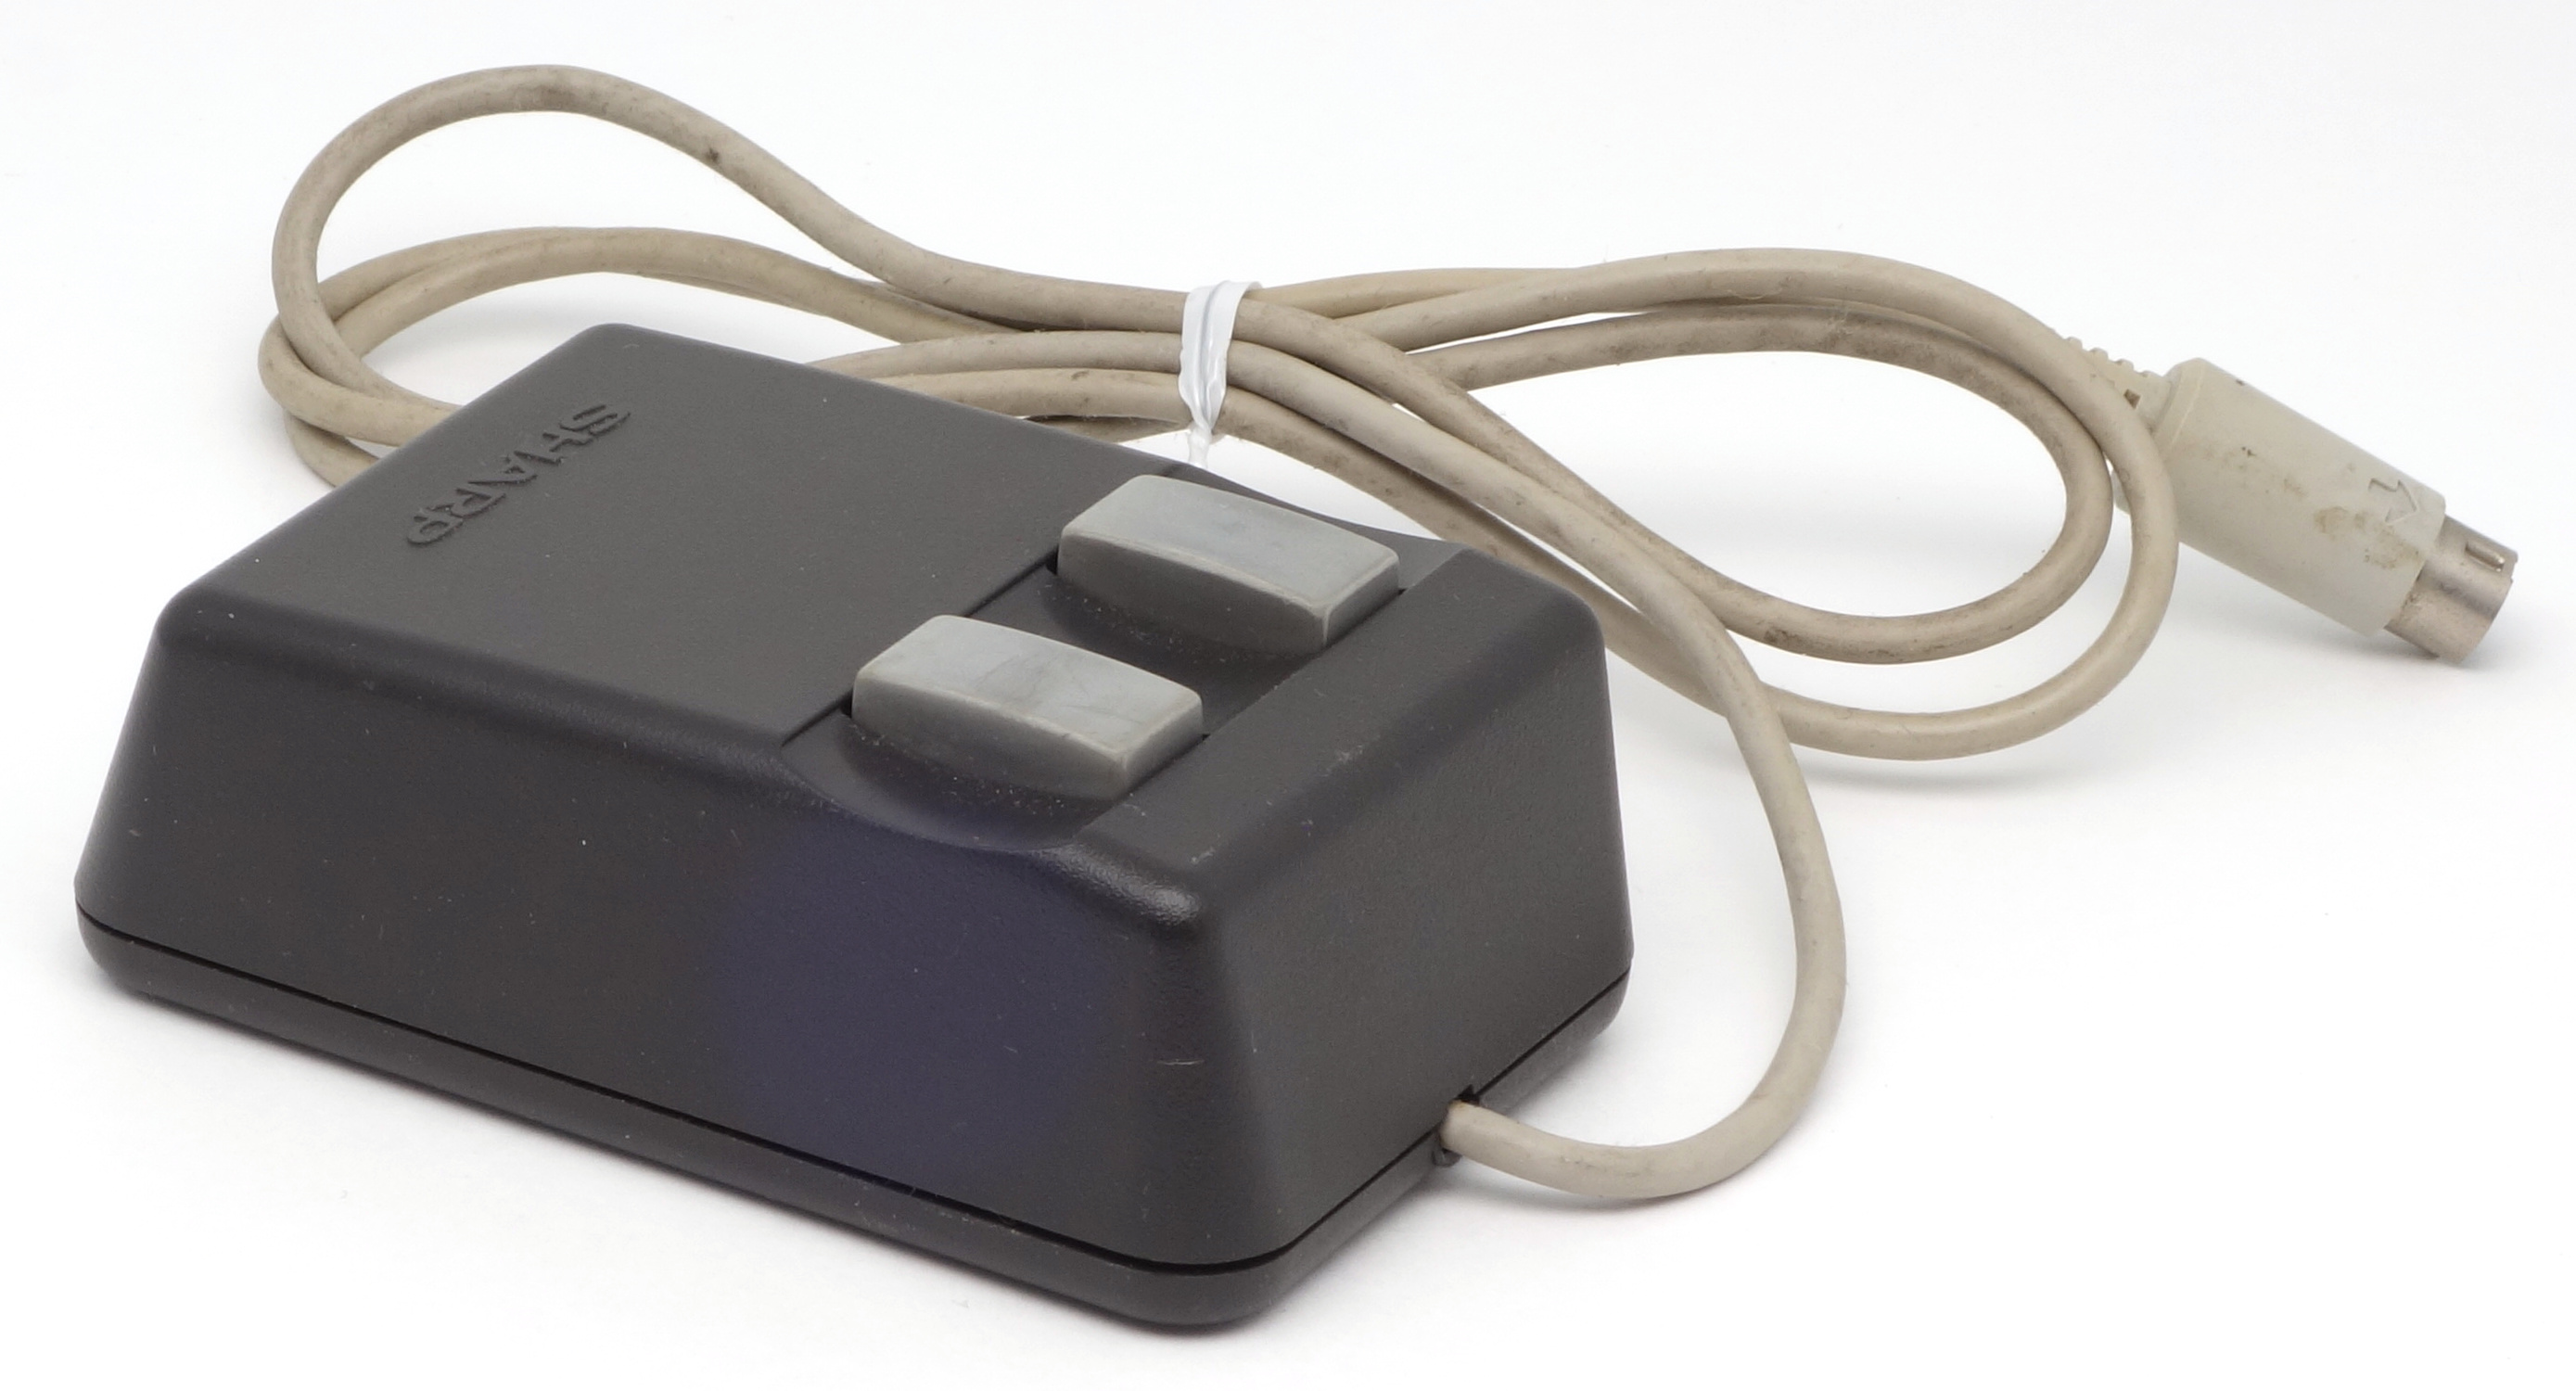
\includegraphics[scale=0.7]{1983_sharp_mz_1x10_mouse/pic_30.jpg}
    \caption{Sharp MZ-1X10 Mouse}
    \label{fig:SharpMZ1x10Pic}
\end{figure}

Корпус мыши MZ-1X10 представляет собой параллелепипед со слегка скругленными гранями и парой прямоугольных кнопок на верхней стороне корпуса (рис.  \ref{fig:SharpMZ1x10Pic}). 
\begin{figure}[h]
    \centering
    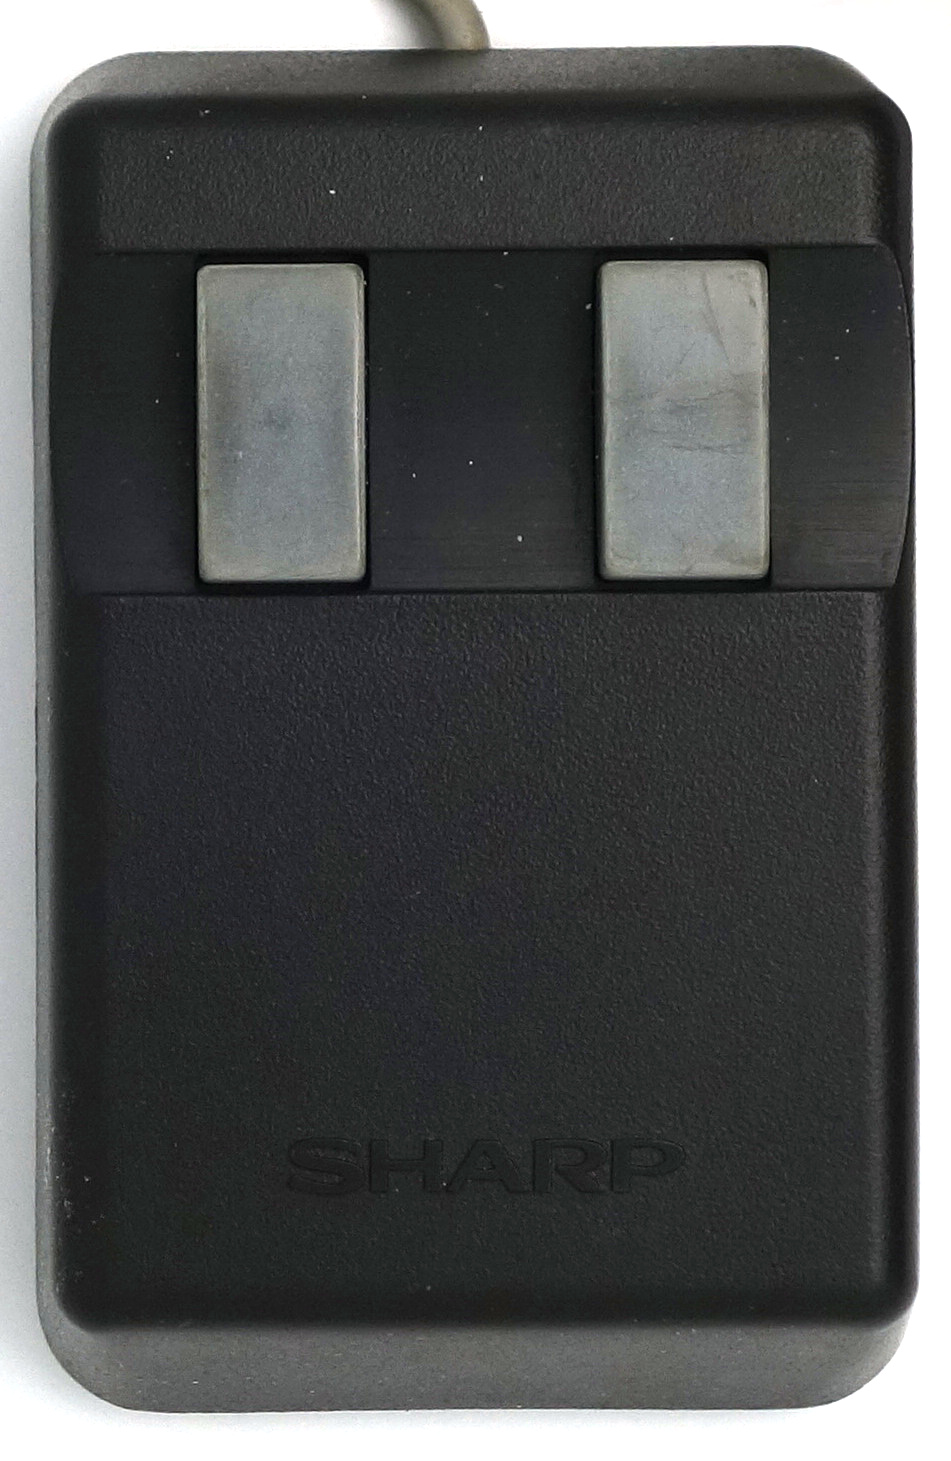
\includegraphics[scale=0.55]{1983_sharp_mz_1x10_mouse/top_15.jpg}
    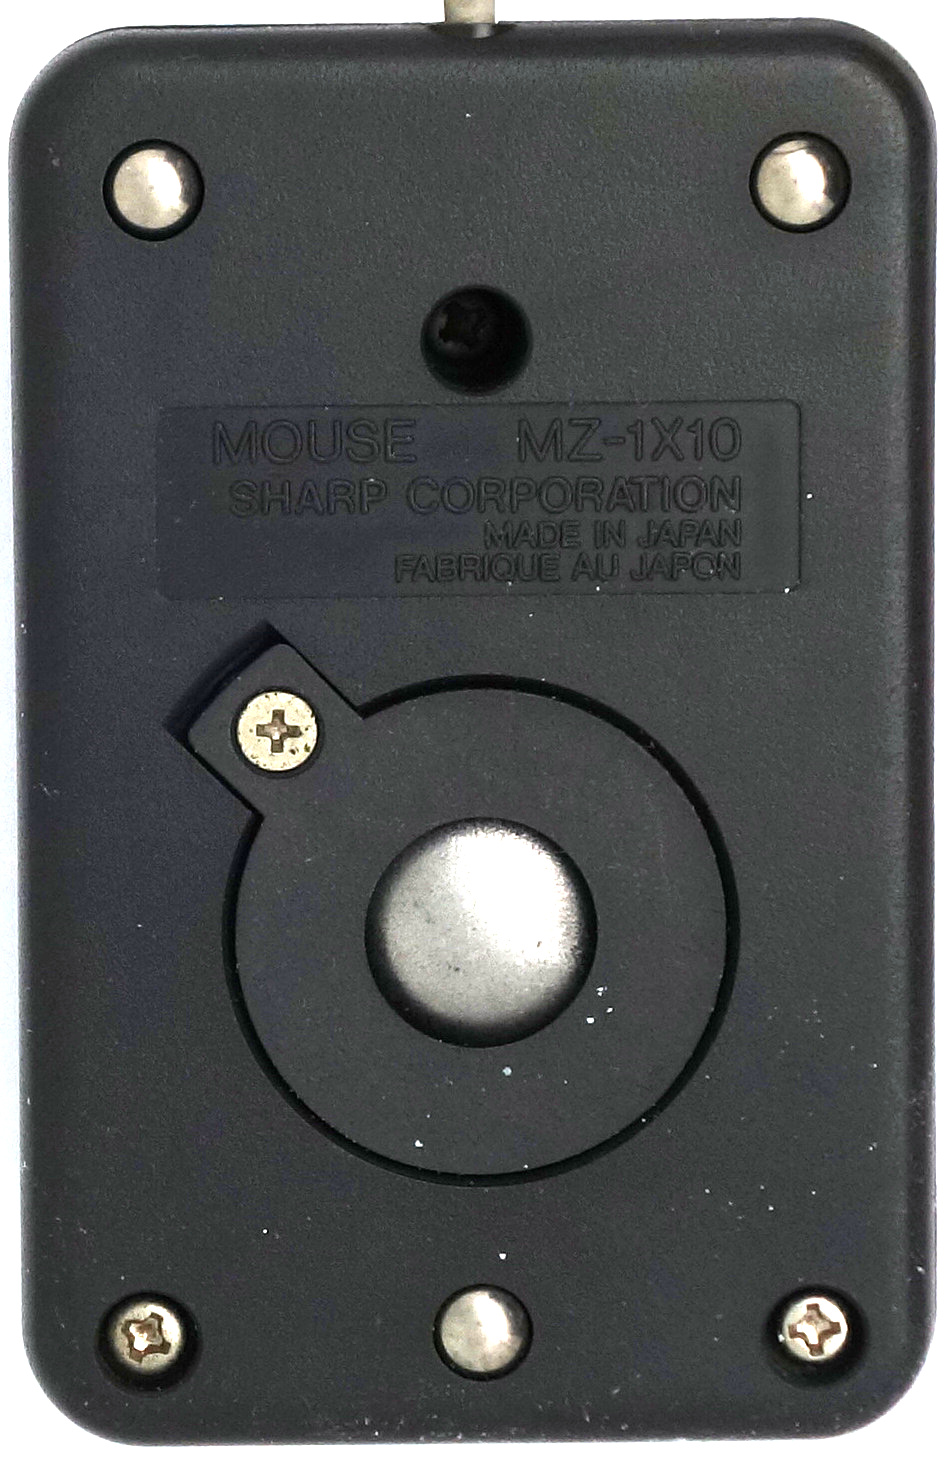
\includegraphics[scale=0.55]{1983_sharp_mz_1x10_mouse/bottom_15.jpg}
    \caption{Sharp MZ-1X10 Mouse, вид сверху и снизу}
    \label{fig:SharpMZ1x10TopAndBottom}
\end{figure}

Нижняя сторона демонстрирует стальной шар, три металлических шарика, облегчающие скольжение мыши, и съёмное кольцо, позволяющее извлечь шар для чистки. Вариант кольца на защелках еще не был придуман, поэтому его требуется отвинчивать с помощью отвертки. Пластиковый ограничитель, защищающий провод от повреждения в месте его выхода из корпуса мыши, конструкцией не предусмотрен (рис. \ref{fig:SharpMZ1x10TopAndBottom}).

\begin{figure}[h]
    \centering
    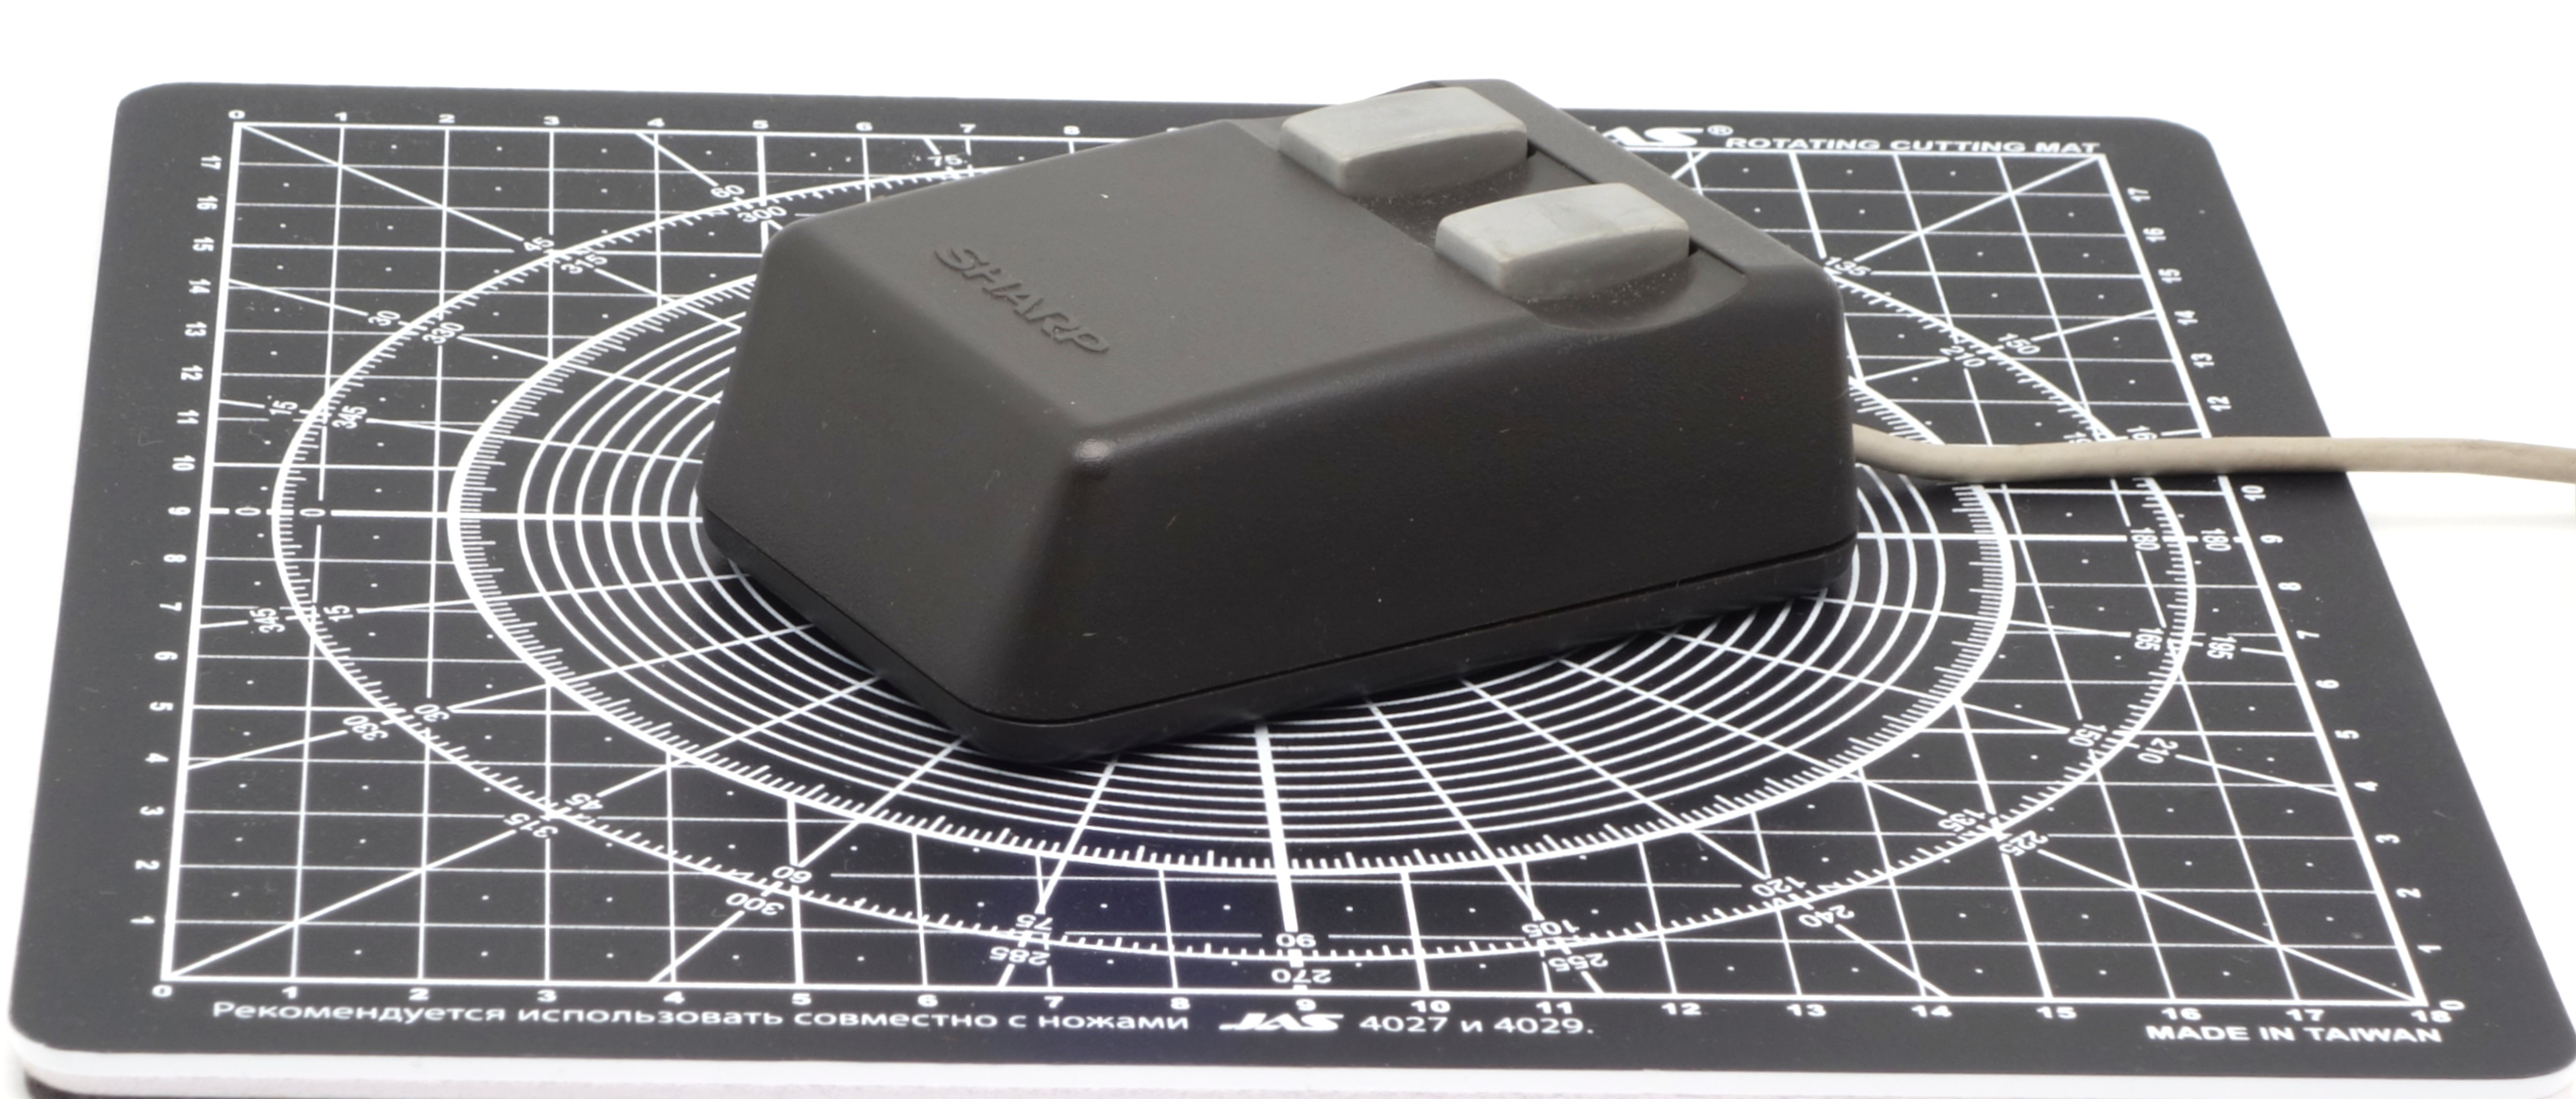
\includegraphics[scale=0.5]{1983_sharp_mz_1x10_mouse/size_30.jpg}
    \caption{Sharp MZ-1X10 Mouse на размерном коврике с шагом сетки 1~см}
    \label{fig:SharpMZ1x10Size}
\end{figure}

Несмотря на малые размеры мыши (рис. \ref{fig:SharpMZ1x10Size}), она довольно тяжелая. Дизайн мыши предельно аскетичен, форма ассоциируется с блоком питания домашних плееров и некоторых других бытовых устройств соответствующего временного периода (либо, благодаря специфическим кнопкам, с автоматическими предохранителями сетей электроснабжения). Очевидно, скошенная задняя грань должна обеспечить более комфортное расположение ладони, однако с учетом размеров мыши существенных улучшений в эргономику это не привносит (рис. \ref{fig:SharpMZ1x10Hand}). Кнопки имеют средний размер, что является приемлемым в плане комфорта.

\begin{figure}[h]
    \centering
    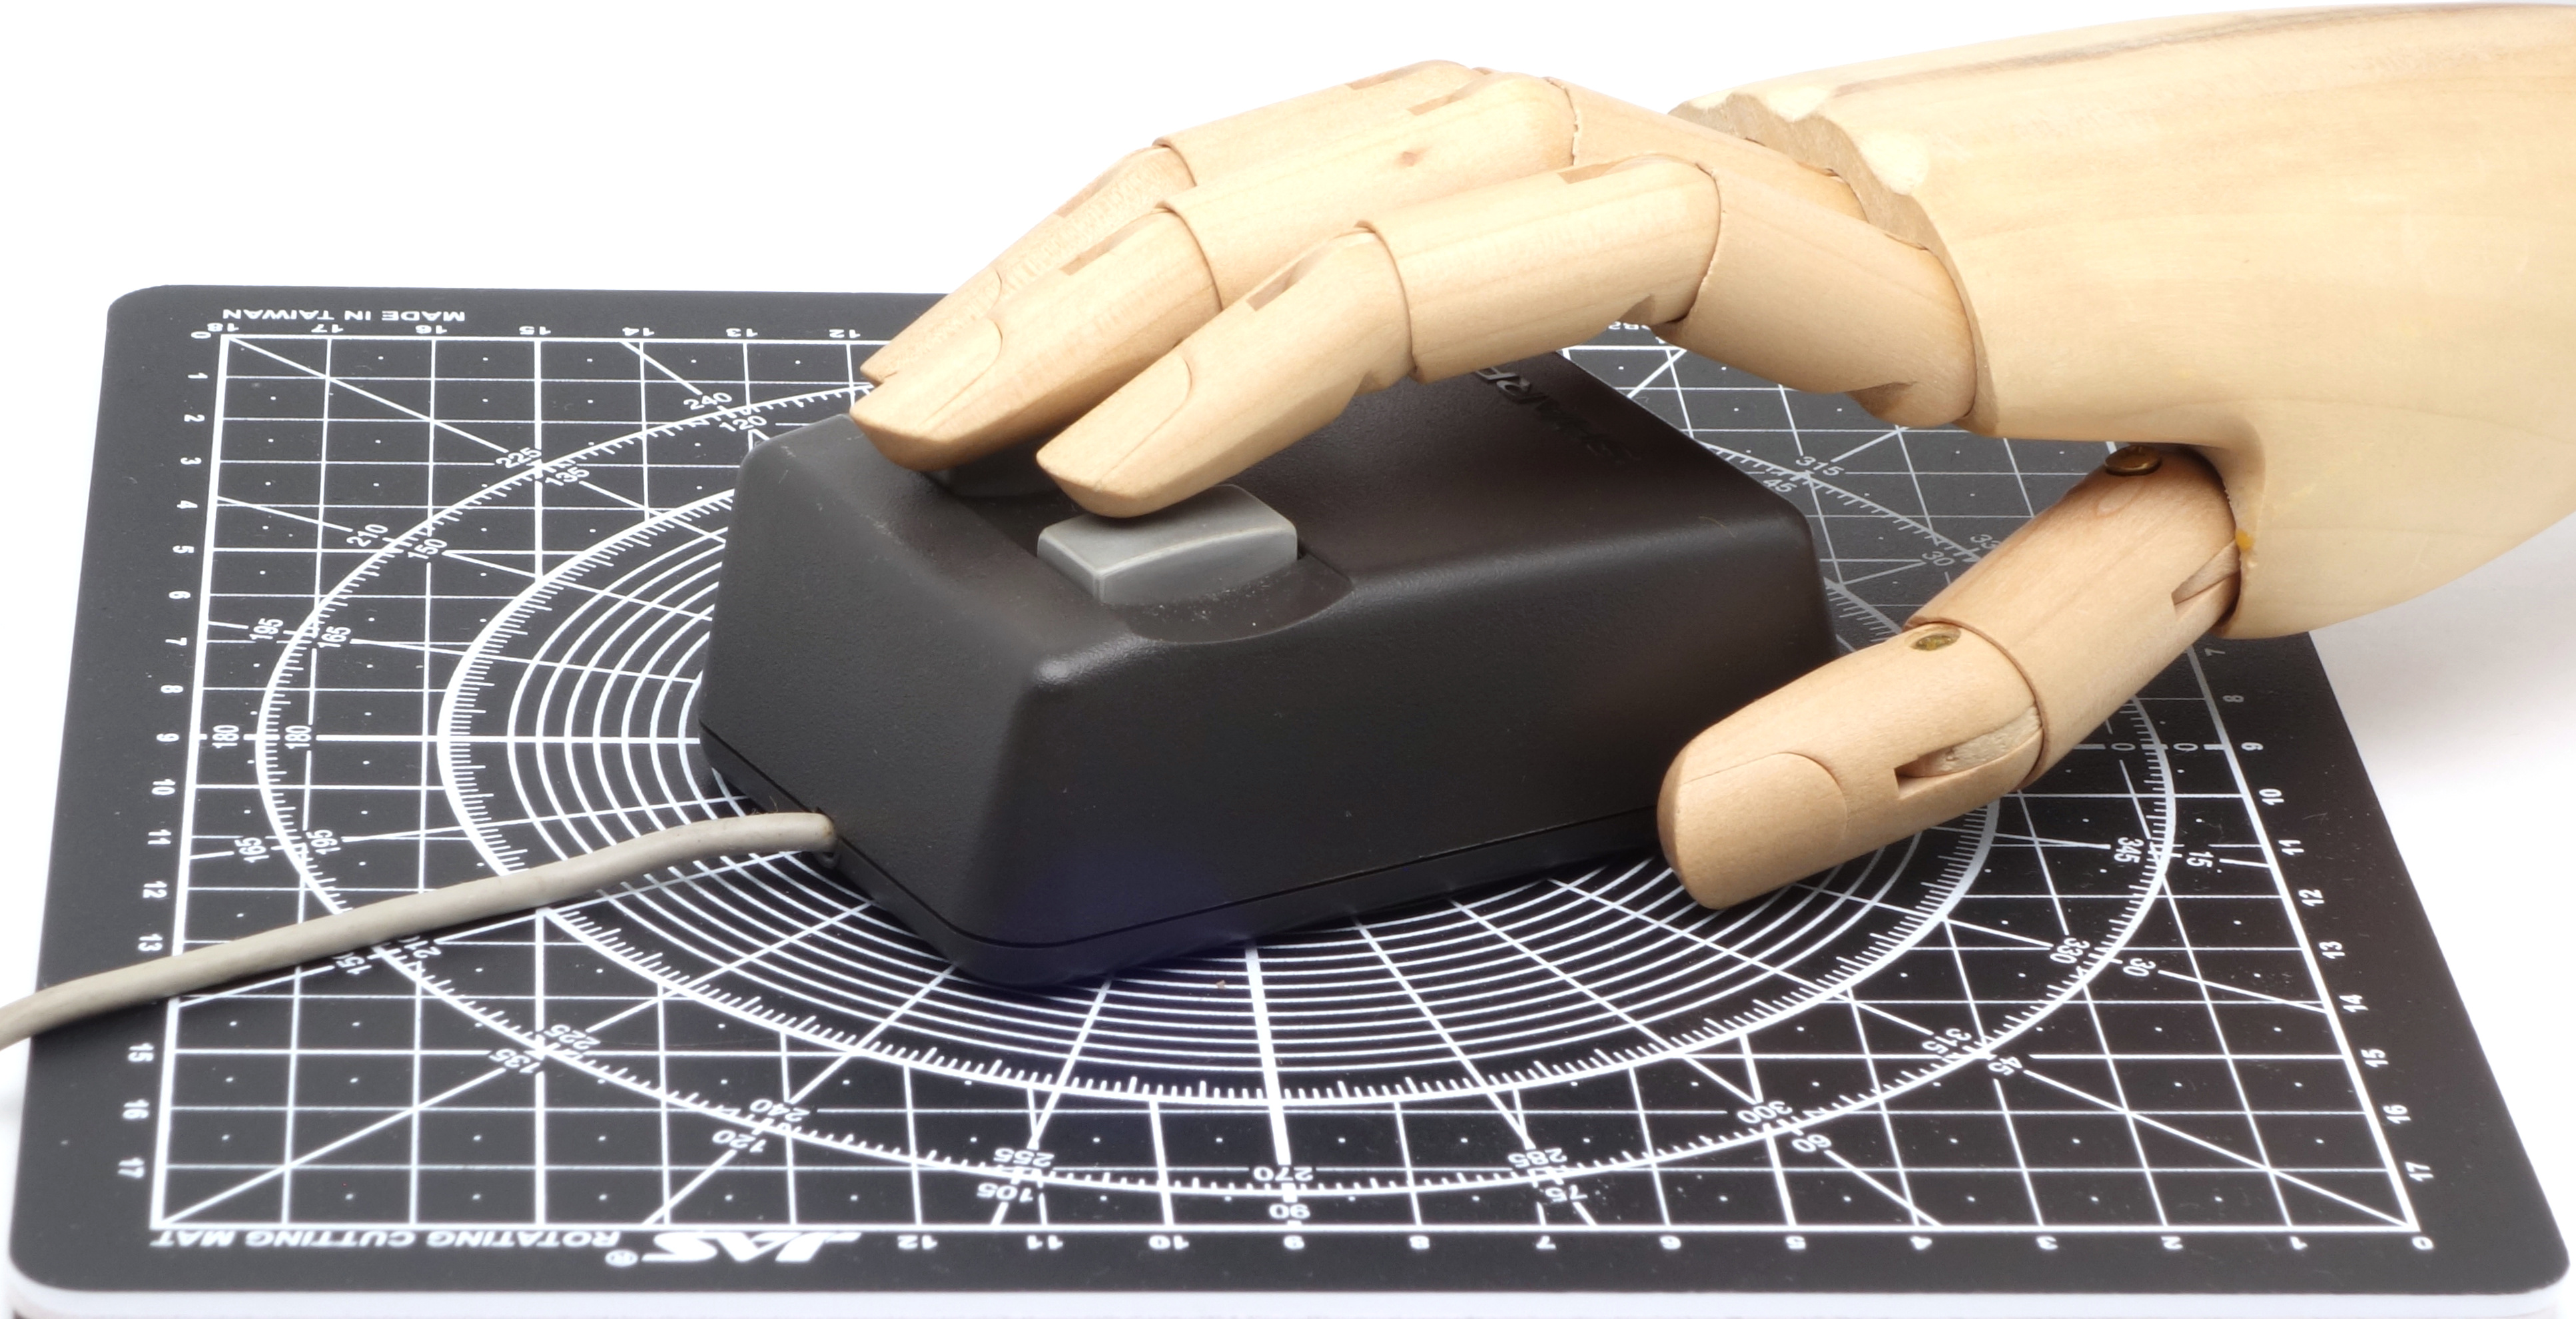
\includegraphics[scale=0.5]{1983_sharp_mz_1x10_mouse/hand_30.jpg}
    \caption{Sharp MZ-1X10 Mouse с моделью руки человека}
    \label{fig:SharpMZ1x10Hand}
\end{figure}

Мышь подключалась к компьютеру по разновидности последовательного интерфейса. Левая кнопка использовалась для возврата к началу координат (левый верхний угол экрана), а правая работала как основная кнопка мыши, то есть генерировала клик в координатах, соответствовавших положению курсора \cite{manual}.

 \begin{figure}[h]
    \centering
    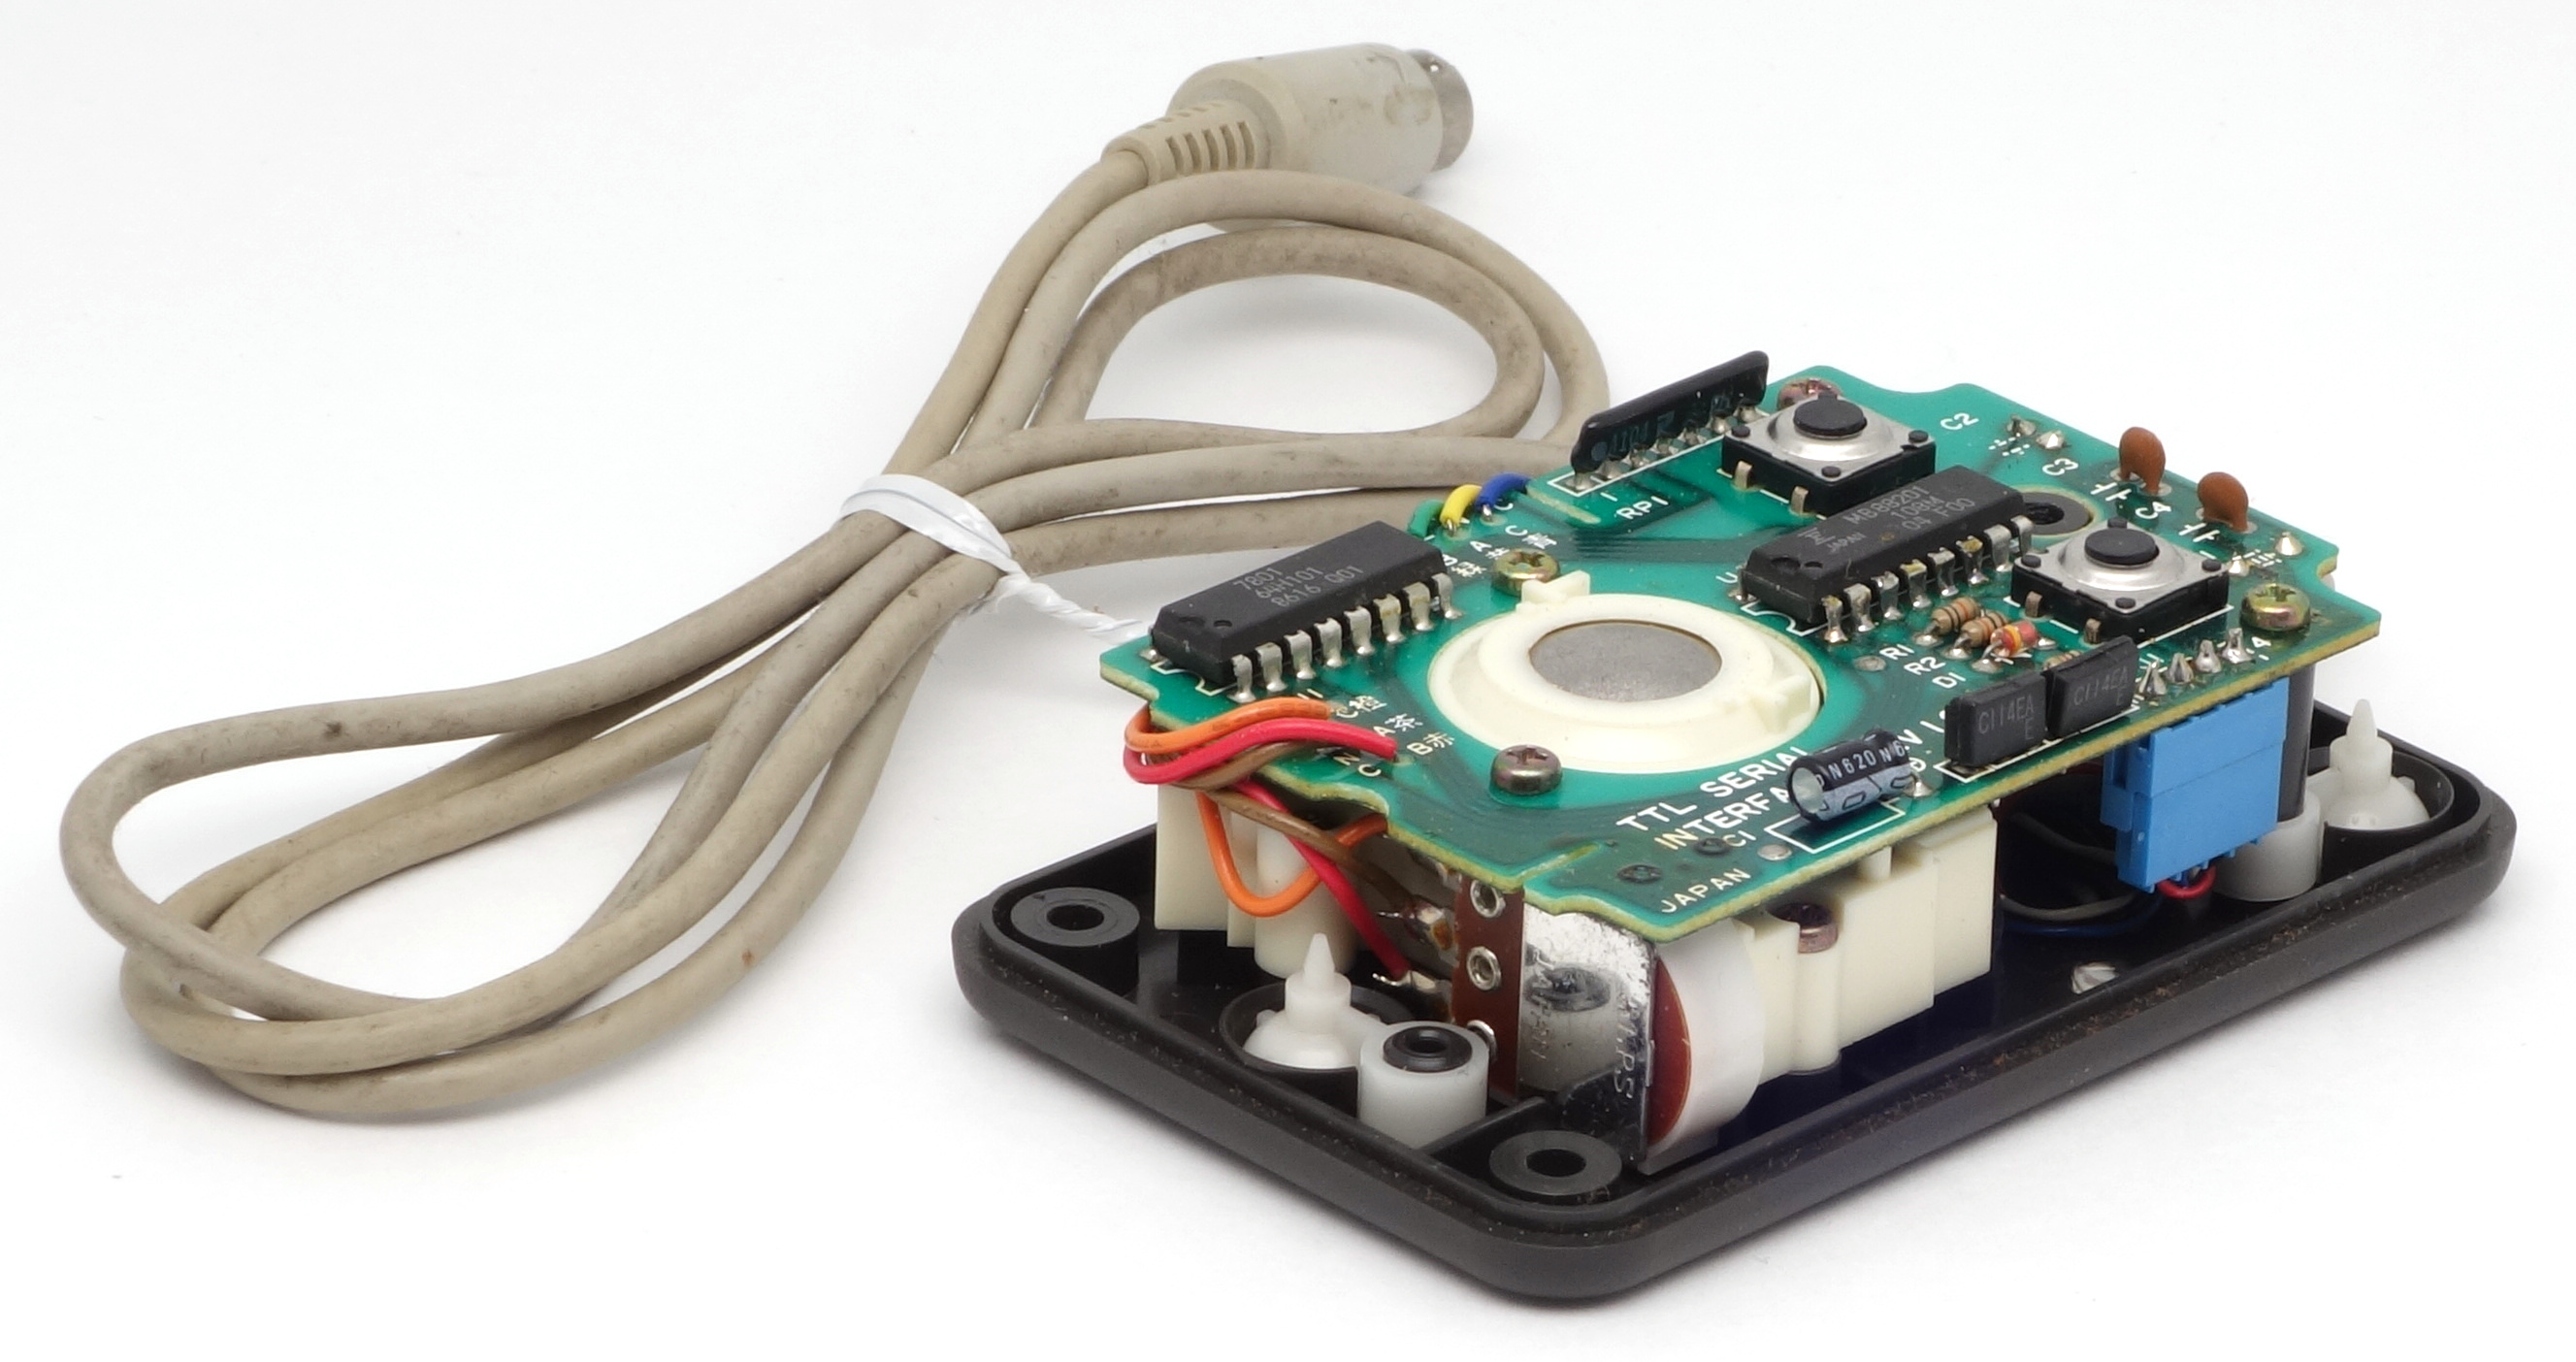
\includegraphics[scale=0.8]{1983_sharp_mz_1x10_mouse/inside_30.jpg}
    \caption{Sharp MZ-1X10 Mouse в разобранном виде}
    \label{fig:SharpMZ1x10Inside}
\end{figure}

Внутреннее устройство мыши показано на рис. \ref{fig:SharpMZ1x10Inside}. В мыши использованы закрытые контактные энкодеры. При сравнении с зеленоглазой мышью Microsoft обнаруживается почти полная идентичность конструкции: отличия наблюдаются в конфигурации печатной платы и связаны с расположением кнопок на верхней стороне корпуса.

\begin{thebibliography}{9}
\bibitem{review}  Ohishi Nobuaki. MZ-1X10 (mouse) [in Japanese] \url{http://retropc.net/ohishi/museum/mz1x10.htm}
\bibitem{wiki} Sharp MZ -- Wikipedia \url{https://en.wikipedia.org/wiki/Sharp_MZ#MZ-3500/5500/6500_group}
\bibitem{manual} Sharp MZ-1X10 Instruction Manual \url{https://www.manualslib.com/download/900861/Sharp-Mz-1x10.html}
\end{thebibliography}
\end{document}
